\chapter{Calibration and Verificiation of Quantum Devices}
\label{ch:QCV}

\section{Introduction}
\label{sec:QCVIntro}
In this chapter, I describe the calibration and testing of a completely
reconfigurable circuit in bulk optics. By altering the parameters in this single
experiment, we were able to simulate the action of any lossless linear optics
circuit on four modes. The architecture was motivated by (but not identical to)
the scheme described by Reck et al in \cite{reck}. An application of this
circuit to quantum simulation is described in chapter~\ref{ch:Simulations}.

\section{Calibration (the crapusoids are real)}
\label{sec:Calibration}
\begin{figure}
  \centering
  \begin{subfigure}{\textwidth}
    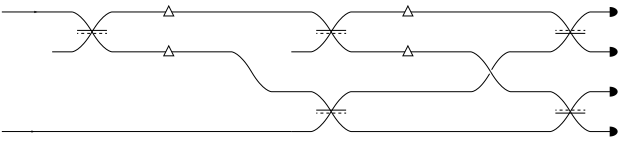
\includegraphics{figures/schematic.pdf}
    \caption{A schematic of the circuit, expanded into path}
    \label{fig:schematic}
  \end{subfigure} \\
  \vspace{1cm}
  \begin{subfigure}{0.45\textwidth}
    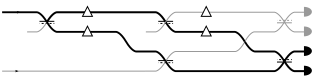
\includegraphics{figures/interferometerAB.pdf}
    \caption{A/B interferometer}
    \label{fig:ab}
  \end{subfigure}
  \hspace{0.05\textwidth}
  \begin{subfigure}{0.45\textwidth}
    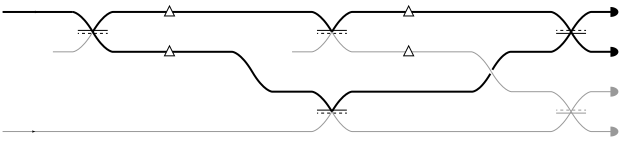
\includegraphics{figures/interferometerCD.pdf}
    \caption{C/D interferometer}
    \label{fig:cd}
  \end{subfigure}
  \caption[Illustration of nested interferometers in the bulk Reck scheme]
  {Interferometers}
  \label{fig:interferometers}
\end{figure}

\section{Benchmarking (the first boson sampler)}
\label{sec:Benchmarking}
Note here that this kind of randomized benchmarking is not always particularly
useful.

\section{Verification}
Work relating to verification in quantum walks and \bosonsampling{}. I don't
think it's unfair to say that I had the original motivation to implement the
\(\rstar\) protocol described in \cite{notuniform}. I did the Bayesian model
comparison between \bosonsampling{} and uniform distributions.

Verifying the output of a Boson sampler brings us up against the notorious
problem of certifying a random number generator based on a short string of
random output. This problem is illustrated in figure:~\ref{fig:dilbert}

\subsection{Is BosonSampling uniform?}
\label{sec:Verification}
\begin{figure}
  \centering
  \includegraphics[width=\textwidth]{figures/protected/dilbert.png}
  \caption[Dilbert discovers that verifying randomness is difficult.]
  {Dilbert discovers that verifying randomness is difficult.}
  \label{fig:dilbert}
\end{figure}

\begin{figure}
  \centering
  \includegraphics{figures/rstar}
  \caption[Using the $\rstar$ discriminator to verify BosonSampling]
  {(a) Expected distribution of \(\rstar\) values when events are sampled
  uniformly (black) and from the full quantum distribution (blue). Experimental
  data from a 3-photon experiment in a 9-mode unitary is shown as a histogram.
  (b) Bayesian model comparison allows real-time updating of our confidence in
  the model describing our data. The models under comparison here are true
  \bosonsampling{} (blue) and uniform sampling (black). We rapidly conclude that
  the data are supported much better by the \bosonsampling{} model.}
\end{figure}

\subsection{Bosonic Clouding}
In a multi-photon quantum walk, we observe a phenomenon where photons tend to
appear in nearby output modes. This is distinct from \emph{Bosonic bunching},
where multiple photons appear in the same output mode.

\subsection{Higher photon numbers}
\begin{figure}
  \centering
  \includegraphics{figures/sixphoton}
  \caption[Bayesian model comparison on 6-photon events]
  {Bayesian model comparison using the full pre-calculated 6-photon
  distributions. (a) Events we believe to be quantum. (b) Events we believe to
  be classical. In both cases, our confidence in the model quickly increases.}
  \label{fig:sixphoton}
\end{figure}
I did some verification on 6-photon events in the recent integrated Reck
experiment. With the circuit set to implement the 6-dimensional quantum Fourier
transform, we injected 6 photons in the state \(\ket{3_{1},3_{2}}\) and
performed a Bayesian model comparison between the quantum and classical
distributions. Again, we quickly become very confident that the data are
quantum, as shown in figure~\ref{fig:sixphoton}.
